% Generated by scireport <version> (template generic@1, layout modern@1) from a bundle with manifest sha256 7112702977a0. Do not edit.
\documentclass[10pt]{article}
\usepackage[a4]{scireport-modern}
\hypersetup{pdftitle={Full-kinds report},%
pdfauthor={N. Cardoso},%
pdfkeywords={compat, spec-1.0},%
pdflang={en},%
  pdfcreator={scireport <version>}}
\scsetrunning{compat corpus}{N. Cardoso}{scireport compat corpus, spec 1.0}
\begin{document}
\sccover{compat corpus}{Full-kinds report}{Every v1.0 kind}{N. Cardoso\par }{DATE & 2026-10-09\\VERSION & 1.0.0\\KEYWORDS & compat, spec-1.0\\}

\par{\parskip=0pt\fontsize{7.5}{10}\ttfamily\bfseries\selectfont\color{sc-accent-ink}\sctrackby{12}{ABSTRACT}\par}\vspace{6pt}
{\scmedium\fontsize{13.5}{18}\selectfont\sctrackonby{-1.2}\setlength{\parskip}{9pt}
A report that exercises \textbf{every} kind.}
\clearpage
\scanchor{sc-toc}{Contents}{}%
\scsectiontitle{Contents}
\sctocrow{0}{01}{Values}{a1}

Short \textbf{markdown} text.

\scchapter{01}{Values}{a1}{Values}{0}

{\parskip=2pt\noindent{\bfseries\color{sc-ink}Number:} 1.23 \ensuremath{\pm} 0.01~arcsec\par}

{\fontsize{8}{11}\selectfont\renewcommand{\arraystretch}{1.65}\setlength{\tabcolsep}{6pt}
\setlength{\sctablew}{\scfullwidth}
\begin{longtable}{>{\raggedleft\arraybackslash\fontsize{7.5}{9}\ttfamily\selectfont}p{\dimexpr 0.33333\sctablew-2\tabcolsep-0pt\relax}>{\raggedleft\arraybackslash\fontsize{7.5}{9}\ttfamily\selectfont}p{\dimexpr 0.33333\sctablew-2\tabcolsep-0pt\relax}>{\raggedright\arraybackslash}p{\dimexpr 0.33333\sctablew-2\tabcolsep-0pt\relax}}
\sctoprule
{\fontsize{7}{9}\selectfont\bfseries\color{sc-ink}\sctrackby{8}{\MakeUppercase{ID}}} & {\fontsize{7}{9}\selectfont\bfseries\color{sc-ink}\sctrackby{8}{\MakeUppercase{Redshift}}} & {\fontsize{7}{9}\selectfont\bfseries\color{sc-ink}\sctrackby{8}{\MakeUppercase{label}}} \\
\scheadrule
\endfirsthead
\sctoprule
{\fontsize{7}{9}\selectfont\bfseries\color{sc-ink}\sctrackby{8}{\MakeUppercase{ID}}} & {\fontsize{7}{9}\selectfont\bfseries\color{sc-ink}\sctrackby{8}{\MakeUppercase{Redshift}}} & {\fontsize{7}{9}\selectfont\bfseries\color{sc-ink}\sctrackby{8}{\MakeUppercase{label}}} \\
\scheadrule
\endhead
\sctoprule
\endlastfoot
1 & 0.100 & a \\
\scrowrule
2 & -- & b \\
\scrowrule
3 & 0.300 & c \\
\end{longtable}}
\begin{adjustwidth}{0pt}{-\scoverhang}\vspace{-1pt}\setcounter{table}{0}\captionof{table}{A Parquet table}\end{adjustwidth}

\begin{adjustwidth}{0pt}{-\scoverhang}
\begin{samepage}
\vspace{14pt}\centering
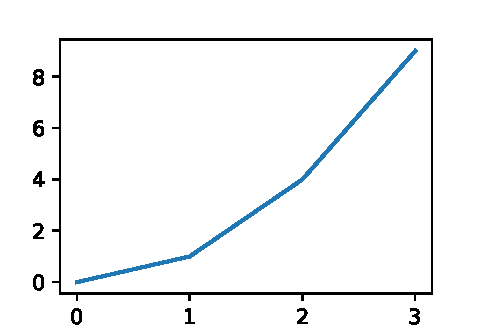
\includegraphics[width=0.6\linewidth]{figures/kinds.figure.pdf}\par\nobreak
% alt: A rising curve
\vspace{7pt}\nobreak\scrule{sc-ink}{0.5pt}\vspace{5pt}\nobreak
\setcounter{figure}{0}\captionof{figure}{y = x squared}
\vspace{12pt}
\end{samepage}
\end{adjustwidth}

\end{document}
